%% LyX 2.0.4 created this file.  For more info, see http://www.lyx.org/.
%% Do not edit unless you really know what you are doing.
\documentclass[oneside,dutch]{amsart}
\usepackage[T1]{fontenc}
\usepackage[latin9]{inputenc}
\usepackage[a4paper]{geometry}
\geometry{verbose,tmargin=3cm,bmargin=3cm,lmargin=2cm,rmargin=2cm}
\setlength{\parskip}{\smallskipamount}
\setlength{\parindent}{0pt}
\usepackage{amsthm}
\usepackage{graphicx}
\graphicspath{{Figures/}}

\makeatletter
%%%%%%%%%%%%%%%%%%%%%%%%%%%%%% Textclass specific LaTeX commands.
\numberwithin{equation}{section}
\numberwithin{figure}{section}

\makeatother

\usepackage{babel}
\begin{document}

\title{Het uitdijend heelal}


\author{N.G. Schultheiss}

\maketitle

\section{Inleiding}

Deze module volgt op de module ``Het heelal''. In deze module wordt
uitgelegd hoe ontdekt is dat het heelal groter wordt. Uiteraard kunnen
we dan ook de gedachte formuleren dat het heelal vroeger kleiner was.
Heel lang geleden was het heelal waarschijnlijk oneindig klein. Dit
idee wordt ook wel de ``The Big Bang'' genoemd.


\section{Vesto Slipher}

Vesto Melvin Slipher deed in eerste instantie spectrografisch%
\footnote{Met een spectrografisch onderzoek bestudeert men de het spectrum kleuren
van een voorwerp.%
} onderzoek aan planeten om de omlooptijd te bepalen. Een aantal planeten
wordt omgeven door een wolkendek. Bij gevolg is het oppervlak niet
te zien en zijn er ook geen duidelijke details waarneembaar. Als we
kunnen kijken hoe snel het gas aan de ene kant naar ons toekomt en
hoe snel het gas aan de andere kant van ons afgaat, kunnen we de omlooptijd
van een planeet bepalen. 

Gelukkig hebben soorten atomen een eigen kleur. Als de atomen van
ons af bewegen verschuift deze kleur naar het rood en als ze naar
ons toe komen verschuift deze kleur naar het violet. Als we de kleurverschuiving
weten, kunnen we de snelheid met het Doppler effect berekenen. Als
we de snelheid weten, kunnen we de omlooptijd van een planeet uitrekenen.

\begin{figure}[h]
\noindent \begin{centering}
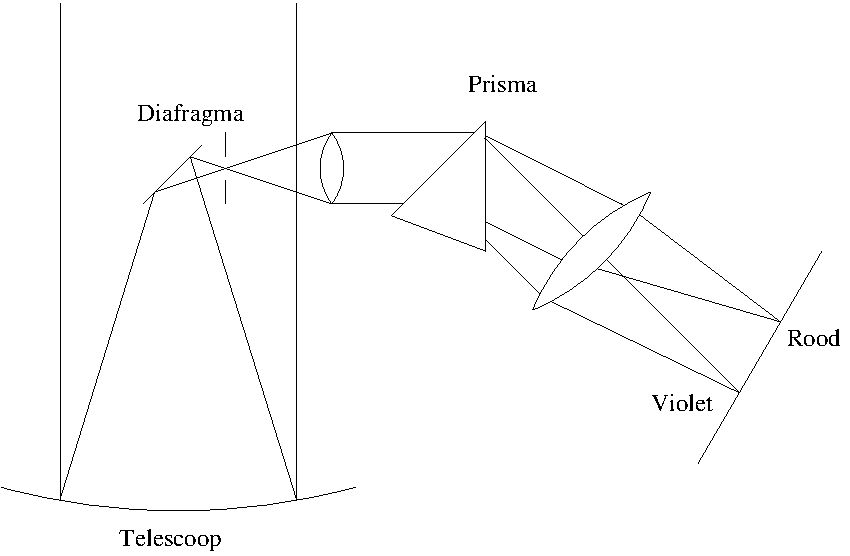
\includegraphics[scale=0.75]{spectrogram}
\par\end{centering}

\caption{Een telescoop met spectroscoop}
\end{figure}


In figuur 2.1 is een opstelling geschetst waarmee de kleurverschuiving
te meten is. In het geval van de reflectie aan een planeet zullen
de atomen hun bijbehorende kleuren absorberen. Dit worden donkere
lijnen in het spectrum tussen rood en violet. In de opstelling kan
het zijn dat het licht van de ene kant van de planeet over het licht
van de andere kant van de planeet wordt afgebeeld. Als we een diafragma
tussen de vlakke spiegel in de telescoop en het oculair van de telescoop
plaatsen, wordt alleen het licht dat we willen meten doorgelaten.
Dit is dan bijvoorbeeld het licht van de linkerkant van de planeet.

In de praktijk is het handiger om een extra lens na de telescoop te
gebruiken. We kunnen dan het diafragma tussen de telescoop en de lens
voor het prisma plaatsen.


\section{Het Doppler effect}

Alle golven en dus ook lichtgolven zijn te defini�ren met twee van
de drie volgende grootheden:
\begin{itemize}
\item De golflengte $\lambda$, deze wordt gemeten in {[}m{]} en geeft aan
hoelang een golf is.
\item De frequentie $f$, deze wordt gemeten in {[}Hz{]} en geeft aan hoeveel
trillingen er in een seconde worden verstuurd in de golf. Bij geluidsgolven
horen we dit aan de toonhoogte, bij lichtgolven zien dit aan de kleur
van het licht. Eventueel is de frequentie ook te berekenen met $f=\frac{1}{T}$,
waarin $T$ de trillngstijd (de duur van 1 trilling) in seconde is.
\item De golfsnelheid $v$, deze wordt gemeten in {[}m/s{]} en geeft aan
hoe snel de golf zich verplaatst. Voor lichtgolven is dit de lichtsnelheid
$c=299792458[\mathrm{m/s}]$.
\end{itemize}
Deze drie grootheden kunnen met de volgende formule gekoppeld worden:

\begin{equation}
v=\lambda f
\end{equation}


Daarnaast komen we ook de grootheid $\phi$ of de fase tegen. Deze
grootheid is een getal en geeft aan hoeveel golven er gepasseerd zijn.
Uiteraard heeft $\phi$ de hoogste waarde bij de bron en de laagste
waarde (0) bij het eerste golffront.

In het geval van geluidsgolven is er geen sprake van relativistische
effecten en kunnen we kijken hoe de frequentie verandert als de bron
met een snelheid $v_{bron}$ beweegt. Voor de geluidssnelheid nemen
we voor de duidelijkheid $v_{geluid}$. In figuur 3.1 is te zien waar
het geluid ($s_{geluid}=v_{geluid}t$) en de bron ($s_{bron}=v_{bron}t$)
op het tijstip \emph{t} zijn.

\begin{figure}[h]
\noindent \begin{centering}
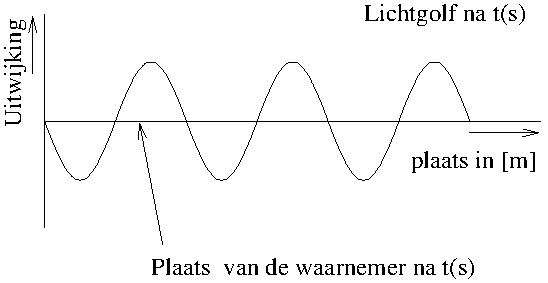
\includegraphics[scale=0.75]{doppler}
\par\end{centering}

\caption{Het Doppler effect voor geluid Galile�-transformatie}
\end{figure}


In figuur 3.1 zien we dat de geluidssnelheid van het geluid ten opzichte
van de waarnemer kleiner is geworden, deze wordt $v=v_{geluid}+v_{bron}$.
Bijgevolg zijn er ook minder fasen langs de waarnemer gekomen. Het
aantal fasen is:

\begin{equation}
\phi_{waarnemer}=\frac{v_{geluid}}{v_{geluid}+v_{bron}}\phi_{geluid}
\end{equation}


Voor de frequentie of het aantal fasen per seconde geldt:

\begin{equation}
f_{waarnemer}=\frac{v_{geluid}}{v_{geluid}+v_{bron}}f_{geluid}
\end{equation}


\begin{equation}
\triangle f=f_{waarnemer}-f_{geluid}=\frac{v_{geluid}}{v_{geluid}+v_{bron}}f_{geluid}-f_{geluid}
\end{equation}


\begin{equation}
\triangle f=\frac{v_{bron}}{v_{geluid}+v_{bron}}f_{geluid}
\end{equation}


Of met licht:

\begin{equation}
\triangle f=\frac{v_{bron}}{c+v_{bron}}f_{licht}
\end{equation}


Zolang de snelheden verwaarloosbaar zijn ten opzichte van de lichtsnelheid,
geldt formule 3.5. Helaas gaat de tijd ook langzamer als de snelheid
in de buurt van de geluidssnelheid komt. Voor snelheden in de buurt
van de lichtsnelheid moeten we nu corrigeren:

\begin{equation}
\triangle f=\left(\sqrt{\frac{c+v_{bron}}{c-v_{bron}}}-1\right)f_{licht}
\end{equation}



\paragraph*{Opdracht 1:}

\emph{Vesto Slipher ontdekte dat de Andromeda-nevel met 300km/s naar
ons toe komt. Onderzoek of deze snelheid het noodzakelijk maakt om
formule 3.6 of formule 3.7 te gebruiken.}


\section{Hubble en Lemaitre}

Edwin Powell Hubble had de beschikking over een 100'' telescoop,
toendertijd was dit de grootste telescoop op Aarde. Doordat deze telescoop
een grote resolutie had kon Hubble waarnemen dat nevels geen nevels
zijn maar sterrenstelsels. Verder nam hij waar dat sterrenstelsels
over het algemeen van ons af bewegen en niet zoals bij de Andromeda-nevel
naar ons toe. 

Verder leek het erop dat hoe verder een sterrenstelsel van ons af
staat, hoe groter de snelheid wordt. De Hubble-constante ligt in de
buurt van de 70{[}km/sMpc{]}. ``Mpc'' staat hier voor Megaparsec.
Omdat een Parsec ongeveer 3.25 lichtjaar is, kunnen we ook zeggen
dat de Hubble constante 21,5{[}km/s{]} per megalichtjaar is.


\paragraph*{Opdracht 2:}

\emph{Het heelal schijnt ongeveer 13,6 miljard jaar oud te zijn. Het
licht kan dus in die tijd maximaal een afstand van 13,6 miljard lichtjaar
afleggen. Bereken met de Hubble constante hoe snel de rand van het
heelal van ons af gaat. Verbaast dit antwoord je?}

Terugredenerend kwam monsigneur Georges Henri Joseph Edouard Lema�tre
tot de conclusie dat er een begin van het heelal moest zijn. Dit idee
werd door diverse wetenschappers zo bizar gevonden dat ze het over
``The Big Bang'' hadden. Tegenwoordig is dit een algemeen aanvaarde
gedachte.


\section{Onderzoek naar de Big Bang}

Als er ooit een Big Bang geweest is, moet dit natuurlijk experimenteel
bevestigd kunnen worden. Vanwege het Doppler effect moeten we dan
naar lange golflengten kijken. Deze liggen in het infrarode gebied
en eventueel zelfs in het gebied van de radiogolven. In 1983 is de
infrarode straling aan de hemel gemeten met de IRAS-satalliet.


\paragraph*{Opdracht 3:}

\emph{Verklaar waarom infrarode straling niet vanaf de Aarde gemeten
kan worden.}


\paragraph*{Opdracht 4:}

\emph{Leg uit waarom men voor een infrarood telescoop een grotere
spiegel nodig heeft dan voor een zichtbaar licht telescoop.}


\paragraph*{Opdracht 5:}

\emph{Leg uit hoeveel maal groter de resolutie van de Hubble-telescoop
(voor zichtbaar licht) is dan de resolutie van de IRAS-telescoop (voor
infrarood licht).}
\end{document}
